\documentclass[12pt]{article}
\usepackage[utf8]{inputenc}
\usepackage{amsmath}
\usepackage{amssymb}
\usepackage{mathtools}
\usepackage{fullpage}
\usepackage[T1]{fontenc}
\usepackage{lmodern}
\usepackage{setspace}
% For fancy math script characters
\usepackage{mathrsfs}
% For aligning long lists in math mode
\usepackage{censor}
\def\censorcolor{white}\let\svcensorrule\censorrule\renewcommand\censorrule[1]{\textcolor{\censorcolor}{\svcensorrule{#1}}}
\usepackage{hyperref}
\hypersetup{
    colorlinks=true,
    linkcolor=blue,
    filecolor=magenta,      
    urlcolor=blue
}
\usepackage{tabularx}
\usepackage{booktabs}
\renewcommand{\arraystretch}{1.5}
\usepackage{multirow}
\usepackage{array}
\usepackage{tikz-qtree}
\usetikzlibrary{calc}
\tikzset{
% Two node styles for game trees: solid and hollow
solid node/.style={circle,draw,inner sep=1.5,fill=black},
hollow node/.style={circle,draw,inner sep=1.5}
}
\usetikzlibrary{matrix}
\usetikzlibrary{fit}
\usetikzlibrary{positioning}
\usepackage[12pt]{moresize}
\usepackage[backend=biber]{biblatex} % load the package
\addbibresource{references.bib} % add a bib-reference file

\title{Probabilistic, Strategic, and Economic Reasoning for Anti-Capitalists}
\author{Jeff Jacobs}

%%% CUSTOM COMMANDS
\newcommand{\Heads}[0]{\textsf{Heads}}
\newcommand{\Tails}[0]{\textsf{Tails}}
\newcommand{\fair}[0]{\textsf{fair}}
\newcommand{\biased}[0]{\textsf{biased}}
\newcommand{\likelihood}[1]{\mathscr{L}\left(#1\right)}
\newcommand{\given}[0]{\; | \;}
\newcommand{\data}[0]{\textsf{data}}
\newcommand{\GoOut}[0]{\textsf{Go Out}}
\newcommand{\StayIn}[0]{\textsf{Stay In}}
\newcommand{\Sunny}[0]{\textsf{Sunny}}
\newcommand{\Rainy}[0]{\textsf{Rainy}}

\newcommand{\strat}[1]{\textsf{#1}}
% Uncomment to make "Corn" have a fancy font
\newcommand{\Corn}[1]{\textsc{corn#1}}
%\newcommand{\Corn}[1]{Corn#1}

\begin{document}

\maketitle

\section*{Introduction}

\doublespacing

If the title of this compendium makes you laugh, you're not alone -- it's probably not clear \textit{a priori} why anti-capitalists would need (much less want) a math book specifically aimed at them. And yet, long story short, I found myself explaining certain ostensibly ``mathematical'' concepts time and time again whole organizing and working with various anti-capitalist, anti-imperialist movements. At a broad level, I also found that these concepts could be classified into three interconnected types:
\begin{itemize}
\item \textbf{Strategic}: \textit{How can we think through our enemy's potential responses to come up with an optimal course of action?},
\item \textbf{Probabilistic}: \textit{How can we assign and compare degrees of belief in the likelihood of these potential responses?}, and
\item \textbf{Economic}: \textit{How can we incorporate the costs and benefits of these actions into our strategic and probabilistic thinking, to better understand what is and isn't feasible?}
\end{itemize}
So I started putting the sections of this thing together so that I could send my written-out explanations to folks rather than ranting about them at some action or post-meeting bar. The concepts in here are variously ``rooted'' in pure math, applied math, probability, statistics, and economics, hence I just chose ``reasoning'' for the title, since despite the importance of the concepts most of those words instill fear and suspicion among leftists that you're a neoliberal or perhaps both.

\section{Week 1: Probabilistic Reasoning}

\subsection{What is a Probability?}

First things first, we need to get some very basic notions of probability down on paper, before we can move into the real meat of the section, Bayesian Statistics. For the purposes of this course, a \textbf{probability} $P(X)$ is just a number between 0 and 1 representing how likely we think some event $X$ is\footnote{If you've taken a stats class in high school or undergrad, you probably learned that a probability $P(X)$ represents ``how likely the event $X$ \textit{is}''. The latter represents the ``frequentist'' philosophy of probability, but in this book we instead adopt a ``Bayesian'' philosophy, which foregrounds the model-builder (you) by treating a probability $P(X)$ as representing ``how likely \textit{we think} the event $X$ is''. Notice the subtle but important difference in wording.}. If we're flipping a coin, for example, and we have no reason to believe that the coin is biased in any way, then we can create and adopt a model of the coin called $\textsf{fair}$ in which $P(\Heads{} \given{} \fair{}) = 0.5$ (read this as ``the probability of seeing heads given the \fair{} model'') and $P(\Tails{} \given{} \fair{}) = 1 - P(\Heads{} \given{} \fair{}) = 0.5$.

As a quick but important aside, the reason we only have to define $P(\Heads{} \given{} \fair{})$ here (with $P(\Tails{} \given{} \fair{})$ being automatically derived as a result) is because the full \textbf{event space} or set of all possible events is $\Omega = \{\Heads{}, \Tails{}\}$. By the rules of probability, $P(\Omega)$ or the probability of \textit{anything} happening:
\begin{align*}
P(\text{Event 1 in  }\Omega\text{ or Event 2 in }\Omega\text{ or Event 3 in }\Omega\text{ or }\ldots)
\end{align*} must equal 1, for a model to be valid\footnote{Hence the equations in this paragraph look like just $P(\textsf{thing})$ rather than $P(\textsf{thing} \given{} \textsf{model})$!}. Then, knowing that the logical connectives ``and'' and ``or'' for events in a valid model must satisfy
\begin{align*}
P(X\text{ and }Y) &= P(X)\cdot P(Y), \\
P(X\text{ or }Y) &= P(X) + P(Y) - P(X\text{ and }Y),
\end{align*}
we know that in any of our models we must have
\begin{align*}
P(\Omega) = P(\Heads{}\text{ or }\Tails{}) &= P(\Heads{}) + P(\Tails{}) - P(\Heads{}\text{ and }\Tails{}) \\
&= P(\Heads{}) + P(\Tails{}) - 0 = 1,
\end{align*}
so that
\begin{align*}
P(\Tails{}) = 1 - P(\Heads{}),
\end{align*}
allowing us to immediately derive $P(\Tails{} \given{} \fair{})$ from our model's assertion that $P(\Heads{} \given{} \fair{}) = 0.5$\footnote{Scrupulous readers will notice that I actually snuck a model assumption into the $P(\Omega)$ line above, namely, that $P(\Heads{}\text{ and }\Tails{}) = 0$. However, if you're that scrupulous hopefully you also know that the ``atomic'' events within $\Omega$ must be mutually exclusive...}. In fact, this gives us a third rule that a valid probability model must satisfy:
\begin{align*}
P(\text{not }X) = 1 - P(X),
\end{align*}
where ``not $X$'' is shorthand for ``the event $X$ does \textit{not} happen''. In our case, since the only two possible events are \Heads{} and \Tails{},
\begin{align*}
P(\Tails{} \given{} \fair{}) = P(\text{not }\Heads{}\given{}\fair{}) = 1 - P(\Heads{} \given{} \fair{}) = 1 - 0.5 = 0.5.
\end{align*}

In the back of our heads, however, we can construct an alternate model of the coin called $\biased{}$, in which $P_\biased{}(\Heads{}) = 0.8$ and $P_\biased{}(\Tails{}) = 1 - 0.8 = 0.2$. Then, the beauty of Bayesian statistics is that we can go out into the world and see which model best comports with what we observe. So, if we notice that the coin keeps coming up heads a suspiciously large number of times, we can change the model we believe from $\fair{}$ to $\biased{}$. Mathematically, we would want to do so if $\likelihood{\data{} \given{} \biased{}} > \likelihood{\data{} \given{} \fair{}}$. This $\mathscr{L}$ thing literally just means ``likelihood'', and it's mathematically the same as probability but written differently to emphasize an unusual property of this calculation: usually when we write $P(X \given{} Y)$ we mean that we're computing $P(X \given{} Y)$ because we want to know how likely $X$ is in a world where we know that $Y$ happened, but in this case we're working ``in reverse'', computing $P(\data{})$ not because we're interested in that quantity in and of itself but only because we want to see how \textit{likely} this outcome was given the (varying) model on the right-hand side of the conditional bar.

\subsection{Optimal Queueing: Why Whole Foods is (Sadly but Truly) the Future}

Now let's apply what we learned in the previous section. Ever notice how, in grocery stores that let you choose which checkout line to wait in, the other lines always seem to go faster than the one you're in? There's a probability-theoretic reason for this! Let's start from the simplest (non-trivial) case: a grocery store with two lines $A$ and $B$. There are only two possibilities here: either $A$ moves faster than $B$, or vice-versa. Mathematically, we can represent this situation by writing out the \textbf{event space} as $\{AB, BA\}$, where the first element represents the case where $A$ moves faster than $B$ and the second elements represents the case where $B$ moves faster than $A$. Without knowing anything about the cashier or the customers in line, the best model we can develop \textit{a priori} is that these two outcomes are equally likely: $P(AB) = P(BA) = 0.5$. So, if you choose to enter line $A$, there's a 50\% chance that your line moves the fastest, and a 50\% chance that the other line $B$ moves the fastest.

So far so good -- the probability that your line moves fastest is the same as the probability that some other line moves fastest. But what happens when we move to a grocery store with 3 lines, $A$, $B$, and $C$? In this case, the possible line orderings (from fastest to slowest) are $\{ABC, ACB, BAC, BCA, CAB, CBA\}$. As before, we consider all of these outcomes as equally likely. So, now what is the probability that the line you choose will be the fastest? If you choose line $A$, your line is the fastest in only two of the six possible outcomes: $ABC$ and $ACB$. Since each outcome is equally likely, each has probability $1/6$, and thus the probability that your line moves fastest, $P(ABC\text{ or }ACB) = P(ABC)+P(ACB)-P(ABC\text{ and }ACB)$, is $1/6+1/6-0 = 2/6$\footnote{Note again that $P(ABC\text{ and }ACB) = 0$, since $ABC$ and $ACB$ are disjoint events -- it can't both be the case that line $B$ moved faster than line $C$ \textit{and} line $C$ moved faster than line $B$.}. Then, using our ``not'' rule from above, the probability that your line does \textit{not} move fastest is
\begin{align*}
1 - P(ABC\text{ or }ACB) = 1 - (2/6) = 4/6.
\end{align*}
So, even with only three lines in the store, we already see that there's only a 33.3\% chance that the line we choose will go the fastest, versus a 66.6\% chance that we will see (at least) one of the other two lines moving faster...

To quickly look at the case of four lines $A$, $B$, $C$, and $D$, note that now the possible events are
\begin{align*}
\Omega &= \{ABCD, ABDC, ACBD, ACDB, ADBC, ADCB, \\
&\censor{= \{}BACD, BADC, BCAD, BCDA, BDAC, BDCA, \\
&\censor{= \{}CABD, CADB, CBAD, CBDA, CDAB, CDBA, \\
&\censor{= \{}DABC, DACB, DBAC, DBCA, DCAB, DCBA\},
\end{align*}
so that whichever line you enter the probability of it being fastest is only $25\%$, and the probability that you will see another line go faster is $75\%$. The logic continues in this way, such that in general if there are $N$ lines the probability that you see another line moving faster than yours is $(N-1)/N$. I used to work as a cashier at a grocery store with 10 checkout lines, putting the probability of frustration for a given customer at an astounding $9/10 = 90\%$... though obviously they all rationally calculated this in their heads and never yelled at me upon seeing one of the 9 other lines moving faster.

\subsection{Bayesian Statistics: A Scary Term for an Intuitive Concept}

One of the scariest sentiments in politics, to me, is the notion that someone or some group ``knows'' that they're ``right'' about something. One of the core principles that sets Marxism or anti-capitalism apart from religion and superstition\footnote{I said it explicitly in the first sentence, but from here on out basically just add ``to me'' to the beginning of all these opinionated statements, in your head. Disclaimer complete.} is the notion that we can come to hold these beliefs by looking out into the world, observing and measuring and comparing things, and updating our beliefs to incorporate whatever we learn. This is the basic intuition behind Bayesian reasoning, which puts this into practice via an ``update equation'' (which you don't have to memorize!) specifying exactly how much one should ``nudge'' their degree of belief in some proposition, thus updating their ``mental model'' of the world, given observed evidence for or against it.

As simple as this seems, it turn out that Bayesian reasoning is \textit{the} optimal method for drawing inferences about social phenomena, In a mathematically-precise sense that we will discuss. For example, a Bayesian gambler will always beat a non-Bayesian given a sufficient number of bets. More on that later.

\subsection{Probabilistic Graphical Models}

“Probabilistic Graphical Model” or PGM is just a fancy term for a statistical tool which operationalizes an intuitive idea: when trying to understand a complex phenomenon with lots of “moving parts” interacting with one another, a good way to start analyzing it is often to break it down into its constituent parts and then specify how these parts work together to give rise to the phenomenon. With this in mind, a PGM is a collection of nodes (drawn as circles) representing variables and edges (drawn as arrows) representing relationships of influence between nodes, codified as “Conditional Probability Tables”. So, if we wanted to model the relationship between weather and a person’s choice of whether to go out and party or stay in and watch a movie on a given Saturday evening, we could use
\begin{enumerate}
\item[(1)] A variable $w$ representing the weather, which can take on values in $\{\Sunny{}, \Rainy{}\}$,
\item[(2)] A variable $a$ representing the person’s action, which can take on values in $\{\GoOut{}, \StayIn{}\}$, and 
\item[(3)] An edge $e$ from $w$ to $a$ which encodes the intuition that one is more likely to go out if it’s sunny than if it’s rainy via the probability distribution $P(a = \GoOut{} | w = \Sunny{}) = 0.8$, $P(a = \StayIn{} | w = \Sunny{}) = 0.2$, $P(a = \GoOut{} | w = \Rainy{}) = 0.1$, and $P(a = \StayIn{} | w = \Rainy{}) = 0.9$, which we can also represent as a simple Conditional Probability Table:
\begin{center}
\begin{tabular}{cc} \hline
Weather (Value of $w$) & Probability of Going Out $P(a=\GoOut{} \; | \; w)$\\ \hline \hline
\Sunny{} & 0.8 \\
\Rainy{} & 0.1 \\\hline
\end{tabular}
\end{center}
\end{enumerate}

We need just one more thing before our PGM is complete, however: while we can use this Conditional Probability Table to obtain any information we want about $a$, notice that the table depends on information about $w$. Thus, to fully parameterize our PGM, we’ll need to supply a non-conditional probability table giving the initial distribution over the weather. In this case, let’s just say that there’s a 50/50 chance of rain or sunshine, so that $P(w = \Sunny{}) = 0.5$.

Now we have everything we need! The resulting PGM, in graphical form, is presented in Figure 3. Pretty boring, but it gets the job done.


\begin{figure}[!ht]
  \centering
  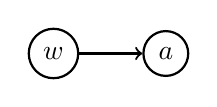
\begin{tikzpicture}[
  %every node/.style={draw, minimum size={width("dmztp")},node distance=0.8cm},
  every node/.style={draw, node distance=0.8cm},
  every path/.style={thick},
  outer/.style={draw,circle},
  inner/.style={draw,circle,minimum size=1cm,inner sep=0},
  metanode/.style={draw,minimum size=3cm,rounded corners=0.4cm},
  obs/.style={fill=lightgray},
  latent/.style={fill=white},
  ar/.style={->,>=latex},
  auto
  ] %
    %\node[outer,obs](w){$w$}; %
    \node[outer](w){$w$};
    \node[outer,right=of w](a){$a$};
    %\node[outer,obs, right=of dyt, xshift=2cm](dztp){$D^z_{t+}$}; %
    \draw[->](w) edge (a);
    %\draw[->](sztp) edge (dztp);
  \end{tikzpicture}
  \label{fig:pgm-noshade}
  \caption{A basic PGM, representing the relationship between $w$, the weather, and $a$, the subsequent action of a person deciding whether to go out or stay in for the night.}
\end{figure}

The beautiful thing about PGMs, though (and the primary reason to use them), is that you can then use this model to make inferences about the world in the face of incomplete information -- i.e., the situation in pretty much every real-world problem. The key tool here is the separation of nodes into two categories: observed (represented graphically as a shaded node) and latent (represented graphically as an unshaded node). Thus we can now use our model as a weather-inference machine: if we observe that the person we’re modeling is out at a party with us, what can we infer from this information about the weather outside? We can draw this situation as a PGM with shaded and unshaded nodes, as in Figure 4, and then use Bayes’ Rule to perform calculations over the network, to see how the observed information about the person at the party “flows” back into the node representing the weather.

\begin{figure}[!ht]
  \centering
  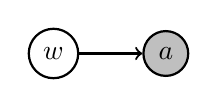
\begin{tikzpicture}[
  %every node/.style={draw, minimum size={width("dmztp")},node distance=0.8cm},
  every node/.style={draw, node distance=0.8cm},
  every path/.style={thick},
  outer/.style={draw,circle},
  inner/.style={draw,circle,minimum size=1cm,inner sep=0},
  metanode/.style={draw,minimum size=3cm,rounded corners=0.4cm},
  obs/.style={fill=lightgray},
  latent/.style={fill=white},
  ar/.style={->,>=latex},
  auto
  ] %
    %\node[outer,obs](w){$w$}; %
    \node[outer](w){$w$};
    \node[outer,obs,right=of w](a){$a$};
    %\node[outer,obs, right=of dyt, xshift=2cm](dztp){$D^z_{t+}$}; %
    \draw[->](w) edge (a);
    %\draw[->](sztp) edge (dztp);
  \end{tikzpicture}
  \label{fig:pgm-shaded}
  \caption{The same situation as in Figure \ref{fig:pgm-noshade}, except that the node for variable $a$ is now shaded, indicating a situation where we have observed the person’s action ($a = Go Out$) but still only have a probability distribution over the weather $w$.}
\end{figure}

Keeping in mind that Bayes’ Rule tells us, for any two events $A$ and $B$, how to use information about $P(B|A)$ to obtain information about $P(A|B)$:
\begin{align*}
P(A|B) = \frac{P(B|A)P(A)}{P(B)},
\end{align*}
We can now apply this rule to obtain our new probability distribution over the weather, taking into account the new information that the person has chosen to go out:
\begin{align*}
P(w = \Sunny{} \; | \; a = \GoOut{}) &= \frac{P(a = \GoOut{} \; | \; w = \Sunny{})P(w = \Sunny{})}{P(a = \GoOut{})} \\
&= \frac{P(a = \GoOut{} \; | \; w = \Sunny{})P(w = \Sunny{})}{P(a = \GoOut{} \; | \; w = \Sunny{}) + P(a = \GoOut{} \; | \; w = \Rainy{})}
\end{align*}

And now we simply plug in the information we already have from our conditional probability table to obtain our new (conditional) probability of interest:
\begin{align*}
P(w = \Sunny{} \; | \; a = \GoOut{}) &= \frac{(0.8)(0.5)}{(0.8)(0.5) + (0.1)(0.5)} = \frac{0.4}{0.4 + 0.05} = \frac{0.4}{0.45} \approx 0.89.
\end{align*}

So we have now learned something interesting from our observation! Namely: now that we’ve observed the person out at a party, the probability that it is sunny out jumps from 0.5 (called the “prior” estimate of the $w$, i.e., our best guess without any other relevant information) to 0.89 (called the “posterior” estimate of $w$)



\section{Strategic Reasoning}

Antonio Gramsci, in his \textit{Prison Notebooks}, made a breakthrough in understanding revolution by disaggregating the Marxian concept of class warfare into two parts: the ``war of maneuver'' and the ``war of position''. The ``war of maneuver'' is the type of thing we imagine when we think of the word ``war'': direct, violent confrontation with the oppressors/exploiters. When the rebels in the Sierra Maestra slowly made their way through Cuba engaging in armed battles against Batista's forces, they were carrying out a ``war of maneuver''. However, as Gramsci argued, a group can't simply get together one day and decide to go ahead and directly confront the exploiters. In any act of revolution, they also need to work to gain a following among the exploited, establishing ``footholds'' among various sectors of society so they have a strong ``position'' in said society from which to attack (hence the name).

In the Russian Revolution, for example, years of organizing and agitation among workers -- who formed the vast majority of the Russian army (just like the US army today) -- ensured that when Kerensky ordered troops to fire upon the Bolsheviks storming the Winter Palace, they refused and abandoned their posts \textit{en masse}. One can see the salience and importance of Gramsci's idea here by imagining what would have happened if the Bolsheviks had ignored the war of position and solely focused on the war of maneuver -- for example, if they had spent all their time doing military drills and studying battlefield maps instead of going across the country organizing future soldiers in their workplaces.

In fact, we don't even have to go back to the 20th century for an example of the crucial role played by the war of position. The 2003 film \textit{The Revolution Will Not Be Televised} documents the attempted US coup against Hugo Chavez in Venezuela, with the camera crew capturing the pivotal moment in the coup's failure when a member of the palace guard suddenly looks over to the camera and holds up a fist. With this gesture, the guard signaled to the millions of protesters outside that that they had not abandoned Chavez and presaged the storming of the Palace by the guards shortly thereafter, driving the US-backed forces out and sounding the death knell for the US's plan.

Thus, at the end of this section, we'll encounter the strategic situation that should be at the front of any anti-capitalist's mind: the ``Revolution Game''. Before we get there, however, we'll need to know the basics. Long story short, unless you end up doing game theory as a profession, you just need to know two standard formats for representing strategic situations: games in ``Normal Form'' and games in ``Extensive Form''.

\subsection{Normal Form Games: Rock, Paper, Scissors}

Normal Form games are the simpler case: essentially they allow us to represent strategic situations where there is a \textit{single} decision that needs to be made, by two or more agents\footnote{Although, above 3 agents the diagrams you'll need to make start looking kinda gross.} who act \textit{simultaneously}. Think Rock, Paper, Scissors: if you were allowed to wait until the other player made a move to choose your own move, the game would be pretty dumb. In fact, let's look at Rock, Paper, Scissors in Normal Form for our first example (I'll explain everything in a minute):

\begin{table}[ht!]
	\centering
	\setlength{\extrarowheight}{2pt}
	\begin{tabular}{cc|c|c|c|}
		& \multicolumn{1}{c}{} & \multicolumn{3}{c}{Column Player ($C$)}\\
		& \multicolumn{1}{c}{} & \multicolumn{1}{c}{\strat{Rock}}  & \multicolumn{1}{c}{\strat{Paper}} & \multicolumn{1}{c}{\strat{Scissors}} \\\cline{3-5}
		\multirow{3}*{Row Player ($R$)}  & \strat{Rock} & $(0,0)$ & $(-1,1)$ & $(1,-1)$ \\\cline{3-5}
		& \strat{Paper} & $(1,-1)$ & $(0,0)$ & $(-1,1)$ \\\cline{3-5}
		& \strat{Scissors} & $(-1,1)$ & $(1,-1)$ & $(0,0)$ \\\cline{3-5}
	\end{tabular}
	\label{fig:rps2}
	\caption{Two-Player Simultaneous Rock, Paper, Scissors game in Normal Form}
\end{table}

The way to read this is, first off, to notice that each row in the matrix (the boxed numbers part) corresponds to one of the moves that the Row Player $R$ can make, while each column corresponds to a move that the Column Player $C$ can make. Thus, the full rules of the game are all there in the cells. To see what happens when Row Player plays Paper while Column Player plays Scissors, for example, we just look at the cell in the Paper ($P$) row and Scissors ($S$) column (2nd row, 3rd column). The two numbers represent the number of points each player gets in this situation, where the first number is how many points Row Player gets and the second is how many points Column Player gets. In our example, since Paper gets cut by Scissors, Row Player loses and gets $-1$ points while Column Player wins and receives $1$ point. If both played Rock instead, the cell at row Rock ($K$) and column Rock ($K$) (1st row, 1st column) tells us that the players both get no points.

We'll learn what we can actually \textit{do} with these matrices soon enough. First, though, note that we can easily extend this format to 3 players: instead of one table we can construct three, and then which of the three we look at is determined by the strategy chosen by Third Player ($T$). Let's make a 3-player version of Rock, Paper, Scissors where you get points based on how you match against two other people. For example, if Third Player plays \strat{Scissors} and the two other players play \textsf{Paper}, Third Player gets two points. But if Third Player plays \textsf{Scissors} while Row Player plays \textsf{Paper} and Column Player plays \textsf{Rock}, then Third Player gets one point for beating Row Player but \textit{loses} one point as well for losing to Column Player. This looks like the following:

\begin{table}
	\centering
	\setlength{\extrarowheight}{2pt}
	\textbf{\underline{(a) Third Player ($T$) chooses \strat{Rock}}}:
	\begin{tabular}{cc|c|c|c|}
		& \multicolumn{1}{c}{} & \multicolumn{3}{c}{Column Player ($C$)}\\
		& \multicolumn{1}{c}{} & \multicolumn{1}{c}{\strat{Rock}}  & \multicolumn{1}{c}{\strat{Paper}} & \multicolumn{1}{c}{\strat{Scissors}} \\\cline{3-5}
		\multirow{3}*{Row Player ($R$)}  & \strat{Rock} & RRR $(0,0,0)$ & RPR $(-1,2,-1)$ & RSR $(1,-2,1)$ \\\cline{3-5}
		& \strat{Paper} & PRR $(-2,1,1)$ & PPR $(1,1,-2)$ & PSR $(0,0,0)$ \\\cline{3-5}
		& \strat{Scissors} & SRR $(-2,1,1)$ & SPR $(0,0,0)$ & SSR $(-1,-1,2)$ \\\cline{3-5}
	\end{tabular}
	
	~\\\rule{0pt}{4ex}
	
	\textbf{\underline{(b) Third Player ($T$) chooses \strat{Paper}}}:
	\begin{tabular}{cc|c|c|c|}
		& \multicolumn{1}{c}{} & \multicolumn{3}{c}{Column Player ($C$)}\\
		& \multicolumn{1}{c}{} & \multicolumn{1}{c}{\strat{Rock}}  & \multicolumn{1}{c}{\strat{Paper}} & \multicolumn{1}{c}{\strat{Scissors}} \\\cline{3-5}
		\multirow{3}*{Row Player ($R$)}  & \strat{Rock} & RRP $(-1,-1,2)$ & RPP $(-2,1,1)$ & RSP $(0,0,0)$ \\\cline{3-5}
		& \strat{Paper} & PRP $(1,-2,1)$ & PPP $(0,0,0)$ & PSP $(-1,2,-1)$ \\\cline{3-5}
		& \strat{Scissors} & SRP $(0,0,0)$ & SPP $(2,-1,-1)$ & SSP $(1,1,-2)$ \\\cline{3-5}
	\end{tabular}
	
	~\\\rule{0pt}{4ex}
	
	\textbf{\underline{(c) Third Player ($T$) chooses \strat{Scissors}}}:
	\begin{tabular}{cc|c|c|c|}
		& \multicolumn{1}{c}{} & \multicolumn{3}{c}{Column Player ($C$)}\\
		& \multicolumn{1}{c}{} & \multicolumn{1}{c}{\strat{Rock}}  & \multicolumn{1}{c}{\strat{Paper}} & \multicolumn{1}{c}{\strat{Scissors}} \\\cline{3-5}
		\multirow{3}*{Row Player ($R$)} & \strat{Rock} & RRS $(1,1,-2)$ & RPS $(0,0,0)$ & RSS $(2,-1,-1)$ \\\cline{3-5}
		& \strat{Paper} & PRS $(0,0,0)$ & PPS $(-1,-1,2)$ & PSS $(-2,1,1)$ \\\cline{3-5}
		& \strat{Scissors} & SRS $(-1,2,-1)$ & SPS $(1,-2,1)$ & SSS $(0,0,0)$ \\\cline{3-5}
	\end{tabular}
	\label{fig:rps3}
	\caption{Three-Player Simultaneous Rock, Paper, Scissors in Normal Form}
\end{table}

As before, the numbers represent the payoffs for the players in each possible outcome. You first use Third Player's chosen action to pick a table, then you find the correct row and column just as before (3rd row, 3rd column). The only difference is the additional 3rd number in the cells now, which represents the payoff for Third Player (with the first two being, as before, Row Player points and Column Player points, in that order). For example, if Row Player plays \strat{Paper}, Column Player chooses \strat{Rock}, and Third Player chooses \strat{Paper}, we look in the 2nd row, 1st column of the 2nd table. We see the payoff profile $(1,-2,1)$, which indicates that Row Player receives 1 point (they beat Column Player's \strat{Rock} with their \strat{Paper} and tied Third Player), Column Player loses 2 points (their \strat{Rock} loses to both the \strat{Paper} chosen by Row Player \textit{and} the \strat{Paper} chosen by Third Player), and Third player receives 1 point (for tying Row Player and beating Column Player's \strat{Rock} with their \strat{Paper}).

If you think about it geometrically, this is equivalent to a $3 \times 3 \times 3$ cube of possible outcomes rather than a $3 \times 3$ square like we had above. Hence since we can imagine 3D cubes, but have a harder time visualizing hypercubes\footnote{Visualizing a 4D hypercube is not too bad if you just imagine a 3D cube with a ``time slider'' underneath it, such that the entries in the cube change as you drag the slider (the cube is ``moving through'' the time dimension). But above that I've got nothing.}, I don't recommend trying to model strategic situations with more than 3 agents this way.

But let's explore another way of representing these types of situations: the Extensive Form. Here I get to use my favorite example, which (I'm sorry) comes from sports: the \href{https://en.wikipedia.org/wiki/Barbados_4\%E2\%80\%932_Grenada_(1994_Caribbean_Cup_qualification)}{1994 Caribbean Cup qualification match} between Barbados and Grenada. The rules in this match were basically the same as standard international-competition rules, with one twist: if the game goes into overtime and a team scores a ``golden goal'' (a goal scored in overtime is ``golden'' in that the game immediately ends and the team who scored wins), they are given \textit{two} points instead of one. As in, if the game was tied 10--10 going into overtime, and the first team scored a goal, the final score would be 12--10. Chaos ensued, however, when Barbados noticed that they were winning 2--1 with only 3 minutes left. It turned out, due to math, that they actually needed to win by \textit{two} points or more in order to advance to the tournament\footnote{The qualifying round of a soccer tournament involves assigning each team to a mini-``league'', where each league has 4 teams total. Every team then plays each other team one time, and after all the games are finished the teams within each league are sorted based on their number of wins, where ties in number of wins are broken based on \textit{goal differential} -- the number of goals a team scored minus the number of goals that were scored on them. This produces the unambiguous final standings of who will enter the subsequent single-elimination tournament and who will not advance.}, because when there are ties with respect to number of wins the teams' goal differentials (number of goals scored minus number of goals given up) are used as the tiebreaker. Noticing this in a galaxy brain moment, Barbados quickly ran over to their own goal and purposefully scored an own-goal. Why? It's time for some game theory folks $\ldots$ Let's map this situation out using the new Extensive Form, which I'll explain in a moment:

~\\

%\begin{tikzpicture}[scale=1.5,font=\footnotesize]
%% Specify spacing for each level of the tree
%\tikzstyle{level 1}=[level distance=15mm,sibling distance=35mm]
%\tikzstyle{level 2}=[level distance=15mm,sibling distance=15mm]
%% The Tree
%\node(0)[solid node,label=above:{Barbados}]{}
%child{node(1)[solid node]{}
	%child{node[hollow node,label=below:{$(a,b)$}]{} edge from parent node[left]{$C$}}
	%child{node[hollow node,label=below:{$(c,d)$}]{} edge from parent node[right]{$D$}}
	%edge from parent node[left,xshift=-3]{$A$}
	%}
%child{node(2)[solid node]{}
	%child{node[hollow node,label=below:{$(e,f)$}]{} edge from parent node[left]{$C$}}
	%child{node[hollow node,label=below:{$(g,h)$}]{} edge from parent node[right]{$D$}}
	%edge from parent node[right,xshift=3]{$B$}
	%};
%\end{tikzpicture}

\begin{figure}
	\centering
	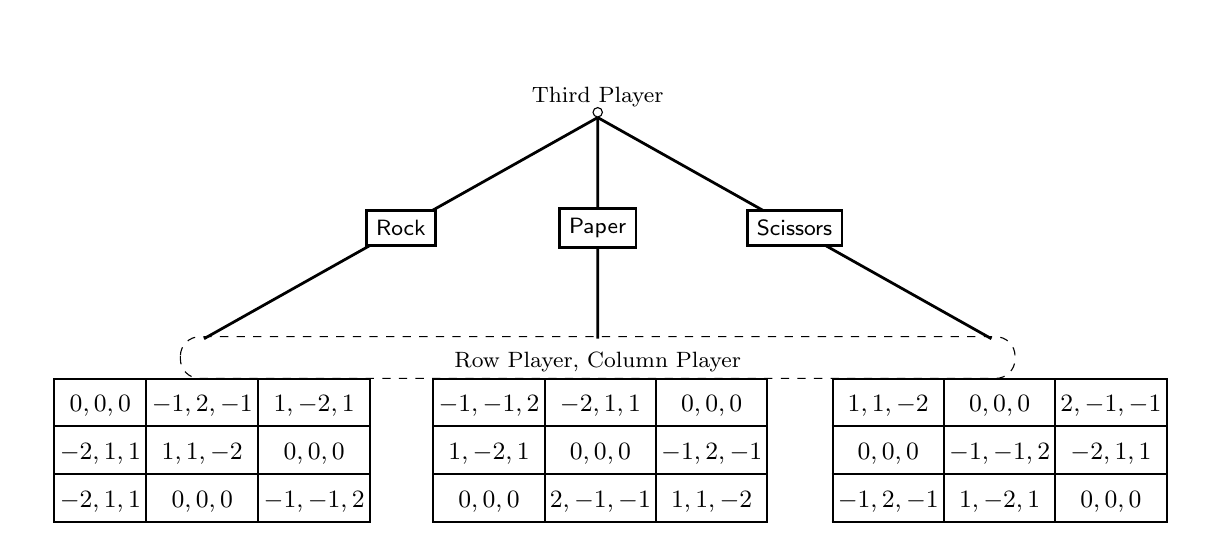
\begin{tikzpicture}[scale=1,font=\footnotesize,edge from parent/.style={line width=1,draw}]
		% Two node styles: solid and hollow
		\tikzstyle{solid node}=[circle,draw,inner sep=1.2,fill=black];
		\tikzstyle{hollow node}=[circle,draw,inner sep=1.2];
		% Specify spacing for each level of the tree
		\tikzstyle{level 1}=[level distance=30mm,sibling distance=50mm]
		\tikzstyle{level 2}=[level distance=30mm,sibling distance=25mm]
		% The Tree
		\node(0)[hollow node]{}
		child{node{}
			edge from parent
			node[line width=1,inner sep=3.5,fill=white,draw=black]{\strat{Rock}}
		}
		child{node{}
			edge from parent
			node[line width=1,inner sep=3.5,fill=white,draw=black]{\strat{Paper}}
		}
		child{node{}
			edge from parent
			node[line width=1,inner sep=3.5,fill=white,draw=black]{\strat{Scissors}}
		};
		\draw[dashed,rounded corners=7]($(0-1)+(-.3,0.15)$)rectangle($(0-3)+(.3,-0.38)$);
		% movers
		\node[above,circle,inner sep=1,yshift=-20]at(0){Third Player};
		\node[below,yshift=-7]at(0-1){
			\arrayrulewidth0.75pt
			\setlength{\tabcolsep}{1.6pt}
			\small{
				\begin{tabular}{|c|c|c|}\hline
					$0,0,0$ & $-1,2,-1$ & $1,-2,1$\\\hline
					$-2,1,1$ & $1,1,-2$ & $0,0,0$\\\hline
					$-2,1,1$ & $0,0,0$ & $-1,-1,2$ \\\hline
			\end{tabular}}
		};
		\node[below,yshift=-7,xshift=-2]at(0-2){
			\arrayrulewidth.75pt
			\setlength{\tabcolsep}{1.5pt}
			\small{
				\begin{tabular}{|c|c|c|}\hline
					$-1,-1,2$ & $-2,1,1$ & $0,0,0$ \\\hline
					$1,-2,1$ & $0,0,0$ & $-1,2,-1$ \\\hline
					$0,0,0$ & $2,-1,-1$ & $1,1,-2$ \\\hline
			\end{tabular}}
		};
		\node[below,yshift=-7]at(0-3){
			\arrayrulewidth.75pt
			\setlength{\tabcolsep}{1.5pt}
			\small{
				\begin{tabular}{|c|c|c|}\hline
					$1,1,-2$ & $0,0,0$ & $2,-1,-1$\\\hline
					$0,0,0$ & $-1,-1,2$ & $-2,1,1$\\\hline
					$-1,2,-1$ & $1,-2,1$ & $0,0,0$\\\hline
			\end{tabular}}
		};
		%\node [circle, draw=black,yshift=-4] at (0-1) {};
		\node[yshift=-5] at ($.333*(0-1)+.333*(0-2)+.333*(0-3)$) {Row Player, Column Player};
	\end{tikzpicture}
	\caption{Simultaneous Rock, Paper, Scissors in Extensive Form\label{fig:simrps}}
\end{figure}

\begin{figure}
	\centering
	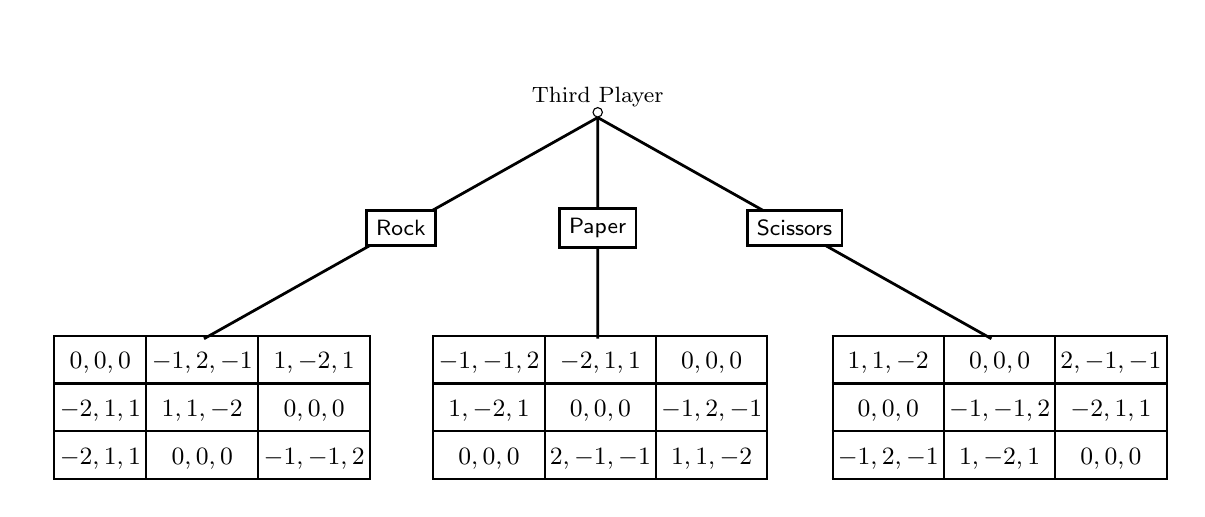
\begin{tikzpicture}[scale=1,font=\footnotesize,edge from parent/.style={line width=1,draw}]
		% Two node styles: solid and hollow
		\tikzstyle{solid node}=[circle,draw,inner sep=1.2,fill=black];
		\tikzstyle{hollow node}=[circle,draw,inner sep=1.2];
		% Specify spacing for each level of the tree
		\tikzstyle{level 1}=[level distance=30mm,sibling distance=50mm]
		\tikzstyle{level 2}=[level distance=30mm,sibling distance=25mm]
		% The Tree
		\node(0)[hollow node]{}
		child{node{}
			edge from parent
			node[line width=1,inner sep=3.5,fill=white,draw=black]{\strat{Rock}}
		}
		child{node{}
			edge from parent
			node[line width=1,inner sep=3.5,fill=white,draw=black]{\strat{Paper}}
		}
		child{node{}
			edge from parent
			node[line width=1,inner sep=3.5,fill=white,draw=black]{\strat{Scissors}}
		};
		% movers
		\node[above,circle,inner sep=1,yshift=-20]at(0){Third Player};
		\node[below,yshift=8.5]at(0-1){
			\arrayrulewidth0.75pt
			\setlength{\tabcolsep}{1.6pt}
			\small{
				\begin{tabular}{|c|c|c|}\hline
					$0,0,0$ & $-1,2,-1$ & $1,-2,1$\\\hline
					$-2,1,1$ & $1,1,-2$ & $0,0,0$\\\hline
					$-2,1,1$ & $0,0,0$ & $-1,-1,2$ \\\hline
			\end{tabular}}
		};
		\node[below,yshift=8.5,xshift=-2]at(0-2){
			\arrayrulewidth.75pt
			\setlength{\tabcolsep}{1.5pt}
			\small{
				\begin{tabular}{|c|c|c|}\hline
					$-1,-1,2$ & $-2,1,1$ & $0,0,0$ \\\hline
					$1,-2,1$ & $0,0,0$ & $-1,2,-1$ \\\hline
					$0,0,0$ & $2,-1,-1$ & $1,1,-2$ \\\hline
			\end{tabular}}
		};
		\node[below,yshift=8.5]at(0-3){
			\arrayrulewidth.75pt
			\setlength{\tabcolsep}{1.5pt}
			\small{
				\begin{tabular}{|c|c|c|}\hline
					$1,1,-2$ & $0,0,0$ & $2,-1,-1$\\\hline
					$0,0,0$ & $-1,-1,2$ & $-2,1,1$\\\hline
					$-1,2,-1$ & $1,-2,1$ & $0,0,0$\\\hline
			\end{tabular}}
		};
	\end{tikzpicture}
	\caption{Sequential Rock, Paper, Scissors in Extensive Form\label{fig:seqrps}}
\end{figure}

%%%%%
%%% Barbados game
%%%%%

\begin{figure}
	\centering
	\begin{tikzpicture}[scale=1,font=\footnotesize,edge from parent/.style={line width=1,draw}]
		% Two node styles: solid and hollow
		\tikzstyle{solid node}=[circle,draw,inner sep=1.2,fill=black];
		\tikzstyle{hollow node}=[circle,draw,inner sep=1.2];
		% Specify spacing for each level of the tree
		\tikzstyle{level 1}=[level distance=30mm,sibling distance=50mm]
		\tikzstyle{level 2}=[level distance=30mm,sibling distance=25mm]
		% The Tree
		\node(0)[hollow node]{}
		child{node{}
			edge from parent
			node[line width=1,inner sep=3.5,fill=white,draw=black]{\strat{Do Nothing}}
		}
		child{node{}
			edge from parent
			node[line width=1,inner sep=3.5,fill=white,draw=black]{\strat{Own Goal}}
		};
		% movers
		\node[above,circle,inner sep=1,yshift=-10]at(0){Barbados};
		\node[below,yshift=-7]at(0-1){
			\arrayrulewidth0.75pt
			\setlength{\tabcolsep}{1.6pt}
			test1
		};
		\node[below,yshift=-7,xshift=-2]at(0-2){
			\arrayrulewidth.75pt
			\setlength{\tabcolsep}{1.5pt}
			test2
		};
		%\node [circle, draw=black,yshift=-4] at (0-1) {};
		\node[yshift=-5] at ($.333*(0-1)+.333*(0-2)+.333*(0-3)$) {Row Player, Column Player};
	\end{tikzpicture}
	\caption{Double Golden Goal Game (Extensive Form)\label{fig:dgg}}
\end{figure}

\subsection{The Revolution Game}

In this game from \cite{mccarty_political_game_theory}, an imperialist country $B$ rules over a colony $A$, and in each ``round'' (here we'll assume a ``round'' spans over the course of 1 year) $A$ and $B$ interact via the following sequential steps (i.e., steps performed in order, such that the actions taken in previous steps are observed/known by whoever is currently making a decision)\footnote{The game ends up pretty much perfectly, though [almost surely] inadvertently, illustrating Gramsci's strategic dichotomy. I've changed the descriptions only a tiny bit here, to match up with the context of the chapter, since (e.g.) the book does not ever cite or mention Gramsci.}:
\begin{enumerate}
	\item A revolutionary group in the colony (which we'll metonymically just also call $A$, for better or worse) decides whether to Revolt and storm the palace ($R$) this year, or to Continue agitating among the population ($C$) during the year, and then
	\item Officials in the metropole (who we similarly refer to as $B$) decide upon a response as follows (based on $A$'s choice):
	\begin{enumerate}
		\item If $A$ chose to Revolt, they decide between caving in and Granting independence ($G$) or violently Suppressing the revolt ($S$).
		\item If $A$ chose to Continue agitating, they decide whether to continue Taxing the colonial population ($T$) or to Eliminate taxes as a preventative measure to lower the (immediate) likelihood of revolt.
	\end{enumerate}
\end{enumerate}
The interesting thing about this game, however, compared to the Rock, Paper, Scissors games we looked at above, is that the sequential rather than simultaneous nature of the choices here requires that the imperial metropole $B$ come up with a policy specifying what to do in \textit{both} of the cases they might end up in: a ``strategy'' for this game, in $B$'s case, is not just a single action choice or even a probability distribution over action choices (like we saw in the Rock, Paper, Scissors cases) but rather a \textit{conditional} policy stating ``if $A$ chooses Revolt, do $X$, otherwise do $Y$''. Any valid strategy for $B$ in this game takes on this form, with $X$ and $Y$ filled in with particular choices. We can represent these strategies in mathematical shorthand as $\{R \rightarrow X, C \rightarrow Y\}$, so that for example the strategy ``If $A$ chooses Revolt, choose Suppress, otherwise choose continue Taxing'' can be shortened to
\begin{align*}
	\{R \rightarrow S, C \rightarrow T\}.
\end{align*}
Finally, before we can start analyzing the game, we need to specify the payoff profile, i.e., how much utility each agent would receive in every possible outcome.

To start with, the key stakes of the colonial extraction here revolve around control of a lucrative oil field in the colony $B$, which generates 4 utils per year for whoever controls it.

Organizing and carrying out a Revolt costs $A$ one util \textit{if} it is not met with Suppression, but if it is then the Revolt costs $A$ 6 utils, and the Suppression itself costs $B$ 6 utils. In the latter case, the relative strengths of the two armies gives rise to some probability $p$ that the Revolt succeeds, in the sense that $A$ is able to gain control over its oil field (and thus the revenue deriving from it) during the round and no longer has to pay taxes to $B$, with a corresponding probability of $1-p$ that the Revolt fails and $B$ retains control over the oil field and continues to collect taxes from $A$.

In the case where $A$ chooses not to Revolt, $B$ receives 2 utils via taxation (meaning that, at the end of the round, $B$ gains 2 utils while $A$ loses 2 utils) if they decide to Continue taxing $A$, or 0 utils via taxation if they decide to Eliminate the tax. So in total we have four possible outcomes, with the payoff profile as follows:
\begin{itemize}
	\item \textbf{[Outcome $O_1 = (R,G)$] $A$ chooses Revolt, $B$ chooses to Grant independence}: $A$ receives a payoff of $\pi_A(O_1) = 3$ utils (4 utils via oil field revenue minus the 1 util ``spent'' on organizing and carrying out the Revolt) and $B$ receives a payoff of $\pi_B(O_1) = 0$ utils, so that the payoff tuple for this outcome is $\pi(O_1) = (\pi_A(O_1),\pi_B(O_1)) = (3,0)$.
	\item \textbf{[Outcome $O_2 = (R,S)$] $A$ chooses Revolt, $B$ chooses to Suppress the revolt}: Here, as described above, the Revolt succeeds with probability $p$ and fails with probability $1-p$, so that
	\begin{itemize}
		\item In the case where the Revolt succeeds, $A$ successfully derives 4 utils from the newly-controlled oil field revenues, and no longer has to pay a tax to $B$, but still loses 6 utils due to the damage from the Suppression, for a net payoff of $4-6 = -2$ utils. $B$, on the other hand, loses 6 utils ``paying for'' the Suppression and no longer gains any utils from taxation or from the oil fields, resulting in a net payoff of $0-6 = -6$ utils.
		\item In the case where the Revolt fails, $A$ loses 6 utils due to the damage from the Suppression, plus they must continue paying taxes to $A$ and thus lose an additional 2 utils, for a net payoff of $0-8 = -8$ utils. $B$ also loses 6 utils carrying out the Suppression, but gains their usual 4 utils from the oil field revenues and 2 utils from taxation of $B$, for a net payoff of $6-6 = 0$ utils.
	\end{itemize}
	Although we can't derive \textit{numeric} values for the payoff tuple $\pi(O_2) = (\pi_A(O_2), \pi_B(O_2))$ here without knowing the numeric value of $p$, we can leave $p$ as an unknown variable and still derive a useful expression for the payoff tuple by writing these payoffs as a \textit{function} of $p$. To do so we ``re-cast'' the payoff tuple $\pi(O)$, for some outcome $O$, as representing the \textit{expected} amount of utility $A$ and $B$ will receive from outcome $O$\footnote{This ``re-casting'' doesn't affect the deterministic payoff values we've already seen, like those of the previous case $O_1$, since the expected value of a non-random quantity is just the quantity itself, by definition. So for the previous outcome $O_1$, with our new definition of $\pi$, we still have
		\begin{align*}
			\pi(O_1) = (\pi_A(O_1),\pi_B(O_1)) = (E[U_A(O_1)], E[U_B(O_1)]) = (E[3],E[0]) = (3,0).
	\end{align*}}. Then we can compute the payoff tuple values as follows, where we also define a helpful ``indicator variable'' $W$ that just numerically represents whether or not the Revolt was successful by taking on the value 1 if it was and 0 otherwise:
	\begin{align*}
		% expected utility for A
		\pi_A(O_2) = E[U_A(O_2)] &= E[U_A((R,S))] = E[U_A(O_2)\given{}W=1] + E[U_A(O_2)\given{}W=0] \\
		&= P(W=1)\cdot U_A(O_2\given{}W=1) + P(W=0)\cdot U_A(O_2\given{}W=0) \\
		&= p\cdot U_A(O_2\given{} W=1) + (1-p)\cdot U_A(O_2\given{} W=0) \\
		&= p\cdot(-2) + (1-p)\cdot(-8) = -2p - 8 + 8p = 6p - 8, \\
		% expected utility for B
		\pi_B(O_2) = E[U_B(O_2)] &= E[U_B((R,S))] = E[U_B(O_2)\given{}W=1] + E[U_B(O_2)\given{}W=0] \\
		&= P(W=1)\cdot U_B(O_2\given{}W=1) + P(W=0)\cdot U_B(O_2\given{}W=0) \\
		&= p\cdot U_B(O_2\given{} W=1) + (1-p)\cdot U_B(O_2\given{} W=0) \\
		&= p\cdot(-6) + (1-p)\cdot(0) = -6p,
	\end{align*}
	so that now we can write the payoff tuple for this outcome as
	\begin{align*}
		\pi(O_2) = (\pi_A(O_2),\pi_B(O_2)) = (6p-8,-6p).
	\end{align*}
	\item \textbf{[Outcome $O_3 = (C,T)$] $A$ chooses to Continue organizing, $B$ chooses to continue Taxing $A$}: $A$ receives a payoff of $\pi_A(O_3) = -2$ utils (via the 2-util tax levied by $B$), and $B$ receives a payoff of $\pi_B(O_3) = 6$ utils (4 utils from the oil revenues plus 2 utils from the tax levied on $B$).
	\item \textbf{[Outcome $O_4 = (C,E)$] $A$ chooses to Continue organizing, $B$ chooses to Eliminate the tax}: $A$ receives a payoff of $\pi_A(O_4) = 0$ utils (since they no longer have to pay the 2-util tax), and $B$ receives a payoff of $\pi_B(O_4) = 4$ utils (via the revenue from the oil field).
\end{itemize}
With the payoff tuples now defined and computed for every possible outcome, we can create the Extensive Form representation of the game, as illustrated in Figure \ref{fig:revgame-ext}.


\begin{figure}
	\centering
	\begin{tikzpicture}[scale=1,font=\footnotesize,edge from parent/.style={line width=1,draw}]
		% Two node styles: solid and hollow
		\tikzstyle{solid node}=[circle,draw,inner sep=1.2,fill=black];
		\tikzstyle{hollow node}=[circle,draw,inner sep=1.2];
		% Specify spacing for each level of the tree
		\tikzstyle{level 1}=[level distance=30mm,sibling distance=75mm]
		\tikzstyle{level 2}=[level distance=30mm,sibling distance=25mm]
		% The Tree
		\node(0)[hollow node]{}
		child{node{}
			edge from parent
			node[line width=1,inner sep=3.5,fill=white,draw=black]{\strat{Revolt ($R$)}}
		}
		child{node{}
			edge from parent
			node[line width=1,inner sep=3.5,fill=white,draw=black]{\strat{Continue Organizing ($C$)}}
		};
		% movers
		\node[above,circle,inner sep=1,yshift=-10]at(0){Revolutionary Movement $A$};
		\node[below,yshift=-7]at(0-1){
			\arrayrulewidth0.75pt
			\setlength{\tabcolsep}{1.6pt}
		}
		child{node{}}
		child{node{}};
		\node[below,yshift=-7,xshift=-2]at(0-2){
			\arrayrulewidth.75pt
			\setlength{\tabcolsep}{1.5pt}
			test2
		};
		%\node [circle, draw=black,yshift=-4] at (0-1) {};
	\end{tikzpicture}
	\caption{Double Golden Goal Game (Extensive Form)\label{fig:dgg}}
\end{figure}

So, for this game, the structure of the Extensive Form representation actually helps us visualize the ``flow'' of the game, with the vertical ``axis'' representing the passage of time as we move from top to bottom -- unlike in World Cup or Rock, Paper, Scissors games where, frankly, we only looked at their Extensive Form representations so we could start getting comfortable with the idea that games always have more than one possible mode of representation. To drive this point home, though, let's see how we would represent this game in Normal form.

First, 

The game is represented in strategic normal form in Figure \ref{fig:revgame}.

\begin{table}[ht!]
	\centering
	\setlength{\extrarowheight}{2pt}
	\begin{tabular}{cc|c|c|}
		& \multicolumn{1}{c}{} & \multicolumn{2}{c}{Palace Guards ($G$)}\\
		& \multicolumn{1}{c}{} & \multicolumn{1}{c}{Fire ($F$)}  & \multicolumn{1}{c}{Stand Down ($SD$)} \\\cline{3-4}
		\multirow{2}*{Revolutionary Army ($R$)}  & Storm ($S$) & $(-100,100)$ & $(100,90)$ \\\cline{3-4}
		& Organize ($O$) & $(0,0)$ & $(0,0)$ \\\cline{3-4}
	\end{tabular}
	\label{fig:revgame}
\end{table}

\subsection{Rules Without Rulers: The Stoplight Game}

% https://codesachin.wordpress.com/2015/11/11/traffic-lights-and-nash-equilibrium/

I grew up in a (purportedly) ``libertarian'' family, which in America really just means ``we don't like anything the government does, but we like anything a private corporation does''. I was raised to pass a stoplight and immediately think ``arbitrary big government imposition on our lives''! So this particular game blew my mind, and made me wonder (to this very day) what other institutions could be mathematically-justified as improving the welfare of all participants?

Picture yourself in an alternate Hobbesian world in which stoplights have been abolished, and imagine two cars both arriving at an intersection at the same time. By now you know the drill -- we'll model the situation as follows: (1) if both cars go, they crash and both drivers receive -10 utils, (2) if neither car goes, they sit there forever and receive -3 utils from the boredom, and (3) if one car goes but the other doesn't, the car that goes receives $4$ utils for safely getting to their destination, and the other car receives $-1$ utils for having to wait for the other car to go before they could go:
\begin{table}[ht!]
	\centering
	\setlength{\extrarowheight}{2pt}
	\begin{tabular}{cc|c|c|}
		& \multicolumn{1}{c}{} & \multicolumn{2}{c}{Car $B$}\\
		& \multicolumn{1}{c}{} & \multicolumn{1}{c}{Go ($G$)}  & \multicolumn{1}{c}{Don't Go ($D$)} \\\cline{3-4}
		\multirow{2}*{Car $A$}  & Go ($G$) & $(-10,-10)$ & $(4,-1)$ \\\cline{3-4}
		& Don't Go ($D$) & $(-1,4)$ & $(-3,-3)$ \\\cline{3-4}
	\end{tabular}
	\label{fig:stoplight}
\end{table}

So what are the Nash equilibria here? (1) If Car $A$ decides to go, Car $B$'s best response is to not go (and receive $-1$ utils). (2) If Car $A$ decides not to go, Car $B$'s best response is to go (and receive 4 utils). The same logic holds for Car $A$ analyzing Car $B$'s potential moves, resulting in a table that looks like:
\begin{table}[ht!]
	\centering
	\setlength{\extrarowheight}{2pt}
	\begin{tabular}{cc|c|c|}
		& \multicolumn{1}{c}{} & \multicolumn{2}{c}{Car $B$}\\
		& \multicolumn{1}{c}{} & \multicolumn{1}{c}{Go ($G$)}  & \multicolumn{1}{c}{Don't Go ($D$)} \\\cline{3-4}
		\multirow{2}*{Car $A$}  & Go ($G$) & $(-10,-10)$ & $(\underline{\mathbf{4}},\underline{\mathbf{-1}})$ \\\cline{3-4}
		& Don't Go ($D$) & $(\underline{\mathbf{-1}},\underline{\mathbf{4}})$ & $(-3,-3)$ \\\cline{3-4}
	\end{tabular}
	\label{fig:slnash}
\end{table}


\section{Economic Reasoning}

As with the other two ``pillars'' of the book, we're going to approach economic reasoning in an extremely selective and unorthodox manner. Specifically, we're basically only going to learn enough econ to be able to work through and understand the economic arguments within John Roemer's game-changing book \textit{Free to Lose: An Introduction to Marxist Economic Philosophy} (1988). Among other things, this is the first and only text I've ever seen that actually tries to grapple with how to define/understand/model ``exploitation'' in a fully mathematically-principled way\footnote{Well, really this is true of his 1981 book \textit{Analytical Foundations of Marxian Economic Theory}, but \textit{Free to Lose} is the first ``layperson-accessible'' text to grapple with it, as far as I can tell.}. So we'll start by working through his model showing how exploitation can emerge from a simple economy consisting of 10 people deciding how to produce the things they need to live (and how to re-produce the things they need in order to continue this production in the future, as we'll see).

\subsection{The Basic Labor-Corn Model}

Imagine a group of 10 people who suddenly find themselves washed up on a deserted island, each having one tasty ear of corn and nothing else. They realize that they'll need to work a certain amount every day in order to have something to eat daily (and thus in order to not die). After searching the island for a while, they find that there are two ways they can produce more corn:
\begin{itemize}
	\item \textsf{Forage}: Beyond the beach there is a large forest where corn, for some reason, grows sparsely in between the inedible trees, grass, and dirt. This means that if they enter the forest and start searching (regardless of how much corn they already have on-hand), they will emerge from the forest with one new corn per 3 hours of searching. Somehow this proportion is infinitely divisible, such that 1.5 hours of searching will produce $\frac{1}{2}$ of a corn, 1 hour will produce $\frac{1}{3}$, 30 minutes will produce $\frac{1}{6}$, and so on.
	\item \textsf{Factory}: In a clearing within the forest, it turns out, an abandoned corn production factory is still standing and ready to be used. What are the odds? Unlike in the forest, however, here our agents will need to have some corn to start with in order to produce more. Specifically, putting 1 \Corn{} in the input tube and turning a crank for 1 hour produces 2 \Corn{s} gross (1 \Corn{} net)\footnote{The difference between gross and net confuses me to no end no matter how many times I think through it, so I'm including this here in case it helps: \textit{Gross} output refers to how much comes out of the machine in total, ignoring whatever went into it as input beforehand. \textit{Net} output, on the other hand, takes into account the inputs to the process and thus instead represents the amount of \textit{additional} material produced, above and beyond the amount provided as input. So since the \strat{Factory} process requires one corn to be used up as input but spits out two corns at the end, we end up with 2 corns gross but 1 corn net.}. As with \strat{Forage}, this process is infinitely divisible: inputting $\frac{1}{2}$ of a \Corn{} and working for 30 minutes produces 1 \Corn{} gross ($\frac{1}{2}$ \Corn{} net), inputting $\frac{1}{4}$ of a \Corn{} and working for 15 minutes produces $\frac{1}{2}$ of a \Corn{} gross ($\frac{1}{4}$ of a \Corn{} net), and so on.
\end{itemize}

An important point is in order regarding \strat{Factory}, which is due to this model being based on \href{https://en.wikipedia.org/wiki/Leontief\_production\_function}{Leontief Production Functions}. These functions model situations where one cannot arbitrarily increase labor hours or capital input to obtain more production, but instead must increase them in a given proportion. This makes sense if you imagine, for example, someone inputting 1 \Corn{} but not performing any labor and thus seeing no output. Shoving a second \Corn{} into the tube will not increase the output any more, since any amount of \Corn{} only leads to the desired output when combined with a corresponding amount of labor hours.

Mathematically, then, we can write these production functions in the following form. First, we can write the output of the \strat{Factory} technology (in net units of corn produced), as a function of how much corn and labor is supplied to it, as
\begin{align*}
	q_{\strat{Factory}}(c,\ell) = \min{\left\{\frac{c}{1},\frac{\ell}{1}\right\}} = \min\{c,\ell\}.
\end{align*}
Here $q_\strat{Factory}$ represents the (net) quantity of corn produced at the end of the \strat{Factory} production process as a function of $c$ and $\ell$, where $c$ represents the amount of corn put into the \strat{Factory} and $\ell$ represents the number of hours worked on that corn. If the math looks scary, remember that this is just a way for us to write out, in the most general possible terms, the details from the previous paragraphs. For example, if we plug in 1 \Corn{} and 1 hour of labor, we get the expected 1 \Corn{} net, since
\begin{align*}
	q_\strat{Factory}(1,1) = \min\{1,1\} = 1~\Corn{}.
\end{align*}
But recall also that we discussed how putting more corn into the machine without also inputting more labor will fail to increase the amount produced. In fact, that fact ``pops out of'' this mathematical formulation as well: if we input $c = 1$ \Corn{} but $\ell = 0$ hours of labor, we see that the net output is zero, as expected:
\begin{align*}
	q_\strat{Factory}(1,0) = \min\{1,0\} = 0~\Corn{}.
\end{align*}
And as well, like in the example, we are still unable to get any output even if we add a second \Corn{}:
\begin{align*}
	q_\strat{Factory}(2,0) = \min\{2,0\} = 0 ~\Corn{}.
\end{align*}

We can write the production function for the \strat{Forage} technology similarly, as
\begin{align*}
	q_\strat{Forage}(c,\ell) = \frac{1}{3}\ell.
\end{align*}
The absence of $c$ from the right-hand-side makes clear that, although you can take corn into the woods if you want, it plays no role in the \strat{Forage} production technology. As with the \strat{Factory} production function, this function ``implements'' the logic of our description from before: for every three hours you put into \strat{Forage}, you receive one \Corn{} (gross and net), since
\begin{align*}
	q_\strat{Forage}(\cdot, 3) = \frac{1}{3}(3) = 1~\Corn{},
\end{align*}
where the $\cdot$ in the first argument to $q_\strat{Forage}$ just indicates that the amount of corn you bring is irrelevant for the outcome.

\subsection{Equilibria in the Basic Labor-Corn Model}

Now that we understand the options

\subsection{The General Labor-Corn Model}

At this point you might be thinking, okay but are these just cooked-up examples where everything works out the way you want because you got to pick exactly the number of agents and their types? In this section, now that you have the intuition, we'll generalize everything from the previous section and show that all of the interesting dynamics hold for any economy with $N$ agents.

\subsection{Agents On Their Grind in the Labor-Corn Economy}

So, let's imagine ourselves as one of the agents in this economy. Hopefully you're lazy like I am so you can understand the agent preferring to only work just enough to re-generate their one \Corn{} each day, so they can spend the remainder of the day lounging on the beach.

The agent's optimization problem:

\begin{align}
	\text{minimize } & Lx_i + z_i \\
	\text{subject to } & (p-pa)x_i + [p - (pa + L)]y_i + z_i \geq pb \\
	& pax_i + pay_i \leq p\omega_i \\
	& Lx_i + z_i \leq 1 \\
	& x_i > 0 \wedge y_i > 0 \wedge z_i > 0
\end{align}

Given this \textit{individual} optimization problem, we can analyze outcomes in the economy by defining corresponding \textit{aggregate} quantities
\begin{align*}
	x = \sum_{i=1}^N x_i, \; y = \sum_{i=1}^N y_i, \; z = \sum_{i=1}^N z_i
\end{align*}

And a price of corn $p$ represents an equilibrium in this model if, after every agent chooses their production vector $\langle x_i, y_i, z_i\rangle$, the aggregate quantities $x$, $y$, and $z$ satisfy
\begin{align}
	(1-a)(x+y) &\geq Nb \\
	Ly &= z \\
	a(x + y) &\leq \omega
\end{align}

\subsection{Capitalism: Is It Necessarily Exploitative?}

\subsection{Class, Wealth, and Exploitation}

\begin{table}[ht!]
	{\fontsize{10}{10}\selectfont
		\begin{tabularx}{\textwidth}{|p{1.6cm}||p{1.4cm}XXp{1.8cm}XXp{2.2cm}|} \hline
			Production vector $\langle x^i, y^i, z^i\rangle$ & \multicolumn{1}{p{1.4cm}|}{Produces on her own?} & \multicolumn{1}{X|}{Hires others to produce?} & \multicolumn{1}{X|}{Sells her labor power?} & \multicolumn{1}{p{1.8cm}|}{Agricultural term} & \multicolumn{1}{X|}{Industrial term} & \multicolumn{1}{X|}{Post-Industrial term?} & Wealth \\ \hline \hline
			\multicolumn{8}{|c|}{\textbf{Bourgeoisie} (Bosses)} \\ \hline
			$\langle 0, +, 0 \rangle$ & No & Yes & No & Landlord & Pure capitalist & CEO & $\omega^i \geq \frac{b}{\pi}$ \\
			& \multicolumn{7}{c|}{Doesn't need to work at all -- simply provides capital to her workers} \\ \hline
			$\langle +, +, 0 \rangle$ & Yes & Yes & No & Rich Peasant (Kulak) & Small capitalist & Small business owner & $\frac{ba}{1-a} < \omega^i < \frac{b}{\pi}$ \\
			& \multicolumn{7}{c|}{Not enough capital to hire workers to produce full consumption bundle} \\\hline \hline
			%$\langle 0, +, + \rangle$ & No & Yes & Yes & \textit{[suboptimal]} & \textit{[suboptimal]} \\
			\multicolumn{8}{|c|}{\textbf{Petit Bourgeoisie} (Independent/``Yeoman'' Workers)} \\ \hline
			$\langle +, 0, 0 \rangle$ & Yes & No & No & Middle Peasant & Petit bourgeois artisan & Full-time Etsy seller & $\omega^i = \frac{ba}{1-a}$ \\
			& \multicolumn{7}{c|}{Has no boss but also doesn't boss others} \\\hline \hline
			%$\langle +, +, + \rangle$ & Yes & Yes & Yes & a & b \\
			\multicolumn{8}{|c|}{\textbf{Proletariat} (``Typical'' Working-Class Workers)} \\ \hline
			$\langle +, 0, + \rangle$ & Yes & No & Yes & Poor Peasant & Semi-proletarian & Uber driver after work & $0 < \omega^i < \frac{ba}{1-a}$ \\
			& \multicolumn{7}{c|}{Has small plot of land, not enough to fully produce needs; ``Proletarianizing''} \\ \hline
			$\langle 0, 0, + \rangle$ & No & No & Yes & Landless Peasant & Proletarian & Service worker & $\omega^i = 0$ \\
			& \multicolumn{7}{c|}{Nothing but their labor power to sell / nothing but their chains to lose} \\ \hline
			$\langle 0, 0, 0 \rangle$ & No & No & No & \multicolumn{4}{c|}{\textit{(suboptimal, doesn't exist in equilibrium)}} \\
			& \multicolumn{7}{c|}{Produces nothing and starves to death... Rough} \\\hline
		\end{tabularx}
	}
	\caption{A combination and extension of Tables 6.1 and 6.2 from \cite{roemer_free_to_lose}, illustrating the connections which arise endogenously between class, wealth, and exploitation in Roemer's model.}
\end{table}

\section{Strategic Reasoning Under Uncertainty}

Now we reach the holy grail: by combining what we've learned from probability theory and statistics about how to grapple with uncertainty, and what we've learned from game theory about how to model strategic interactions, we can develop a set of principled mathematical frameworks for figuring out what to do in the various highly-uncertain multi-agent situations we find ourselves in when organizing and developing political strategies.

- Game Theory and Mechanism Design for Anti-Capitalists

-- 1. Intro

*Game Theory*: modeling strategic interactions between people. What decision(s) are in this person's best interests, given that they don't know what the other person is going to do?

*Mechanism Design*: "inverse" game theory. Now we get to *create* the game (read: institution) that people will participate in. How can we create "good" games? i.e., how can we create games where good things will happen even if people act like assholes?

First game theory example: [The Evolution of Trust](https://ncase.me/trust/)!

Now do the ones \hyperref{https://cs.stanford.edu/~jjacobs3/Jacobs_GameTheoryAndMechanismDesign.pdf} (slides from Stanford weekend course for high school students)

-- 2. More Intro

Second game theory example: Schelling segregation model. [Parable of the Polygons!](https://ncase.me/polygons/)

First mechanism design example: walk through the steps showing why a first-price auction is *not* a good way to auction an item. Refer to the slides from above

-- 3. Actual, like, society

* Stoplight game


\singlespacing

\nocite{*}

\printbibliography[title={Primary Readings},keyword=primary]
\printbibliography[title={Additional Resources},keyword=secondary]

\end{document}
